\section {Cross Attention}
\label{sec:ca_defn}
%--------------------------------------------------------------------------------------------------
%\paragraph{Cross attention}
Let matrix $F_\ell \in \real^{p_\ell \times d_\ell}$ be a reshaping of feature tensor $\vF_\ell$ at
 layer $\ell$, where $p_\ell \defn w_\ell h_\ell$ is the number of patch tokens without \cls, and
  let $\vq_\ell \in \real^{d_\ell}$ be the \cls token embedding at layer $\ell$. By focusing on the 
  \emph{cross attention} only between the \cls (query) token $\vq_\ell$ and the patch (key) tokens 
  $F_\ell$ and by ignoring projections $W_Q, W_K, W_V$ for simplicity, attention $A$ ~\eq{att} 
  is now a $1 \times p_\ell$ matrix that can be written as a vector $\mathbf{a} \in \real^{p_\ell}$

\begin{equation}
	\mathbf{a} = A\tran = \softmax \left( \frac{F_\ell \vq_\ell}{\sqrt{d_\ell}} \right).
\label{eq:cross-attention}
\end{equation}

\noindent Here, $F_\ell \vq_\ell$ expresses the pairwise similarities between the global \cls feature 
$\vq_\ell$ and the local patch features $F_\ell$. Now, by replacing $\vq_\ell$ by an arbitrary vector 
$\mathbf{a}lpha \in \real^{d_\ell}$ and by writing the feature matrix as $F_\ell = (\vf_\ell^1 \dots 
\vf_\ell^{d_\ell})$ where $\vf_\ell^k = \vect(F_\ell^k) \in \real^{p_\ell}$ for channel $k$, 
attention ~\eq{cross-attention} becomes

\begin{equation}
	\mathbf{a} = h_\ell (F_\ell \mathbf{\alpha}) =
		h_\ell \left( \sum_k \alpha_k \vf_\ell^k \right).
\label{eq:connection}
\end{equation}

\noindent This takes the same form as~\eq{sal}, with feature maps $F_\ell^k$ being vectorized into 
$\vf_\ell^k$ and the activation function is defined as $h_\ell(\vx) = \softmax(\vx / \sqrt{d_\ell})$. 
Eq. ~\eq{connection} is visualized in \autoref{fig:connection}. We thus observe the following.

\begin{quote}
	\emph{Pairwise similarities between one query and all patch token embeddings in cross attention 
	are the same as a linear combination of feature maps in CAM-based saliency maps, where the 
	weights are determined by the elements of the query.}
\end{quote}

\noindent As it stands, one difference between~\eq{sal} and~\eq{connection} is that~\eq{connection} 
is class agnostic, although it could be extended by using one query (weight) vector per class. For 
simplicity, we choose the class agnostic form in the following. %We also choose to have no query/key projections. 
%However, we do provide additional experiments with class specific representation as well as projections
% in \autoref{sec:gen_ablation}. 
%--------------------------------------------------------------------------------------------------
\paragraph{Pooling, or masking}
We are thus motivated to integrate an attention mechanism into any network such that making a 
prediction and explaining (localizing) it are inherently connected. In particular, considering 
cross attention only between \cls and patch tokens~\eq{cross-attention}, equation~\eq{SA} becomes

\begin{figure}[t]
    \centering
    % editable at https://docs.google.com/drawings/d/1nfqVV_dNqSV9g5UBuNopPLvubcEZx-vvg4K0ZCvNdfU/edit
    %\fig[.7]{CA-CAM}
    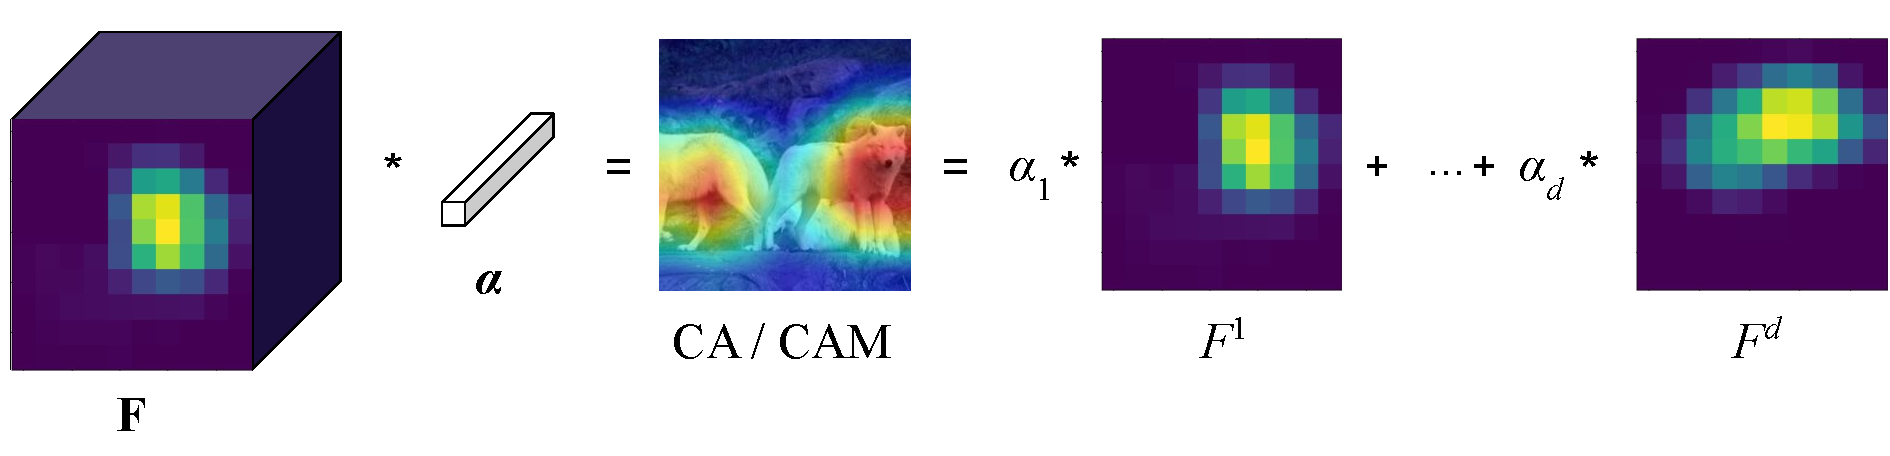
\includegraphics[width=.7\textwidth]{fig/castream/images/CA-CAM.pdf}
    \vspace{3pt}
    \caption{}
    %\emph{Visualization of eq.~\eq{connection}.} On the left, a feature tensor $\vF \in \real^{w \times h \times d}$ is multiplied by the vector $\valpha \in \real^d$ in the channel dimension, like in $1 \times 1$ convolution, where $w \times h$ is the spatial resolution and $d$ is the number of channels. This is \emph{cross attention} (CA)~\cite{dosovitskiy2020image} between the query $\valpha$ and the key $\vF$. On the right, a linear combination of feature maps $F^1, \dots, F^d \in \real^{w \times h}$ is taken with weights $\alpha_1, \dots, \alpha_d$. This is a \emph{class activation mapping} (CAM)~\cite{zhou2016learning} with class agnostic weights. Eq.~\eq{connection} expresses the fact that these two quantities are the same, provided that $\valpha = (\alpha_1, \dots, \alpha_d)$ and $\vF$ is reshaped as $F = (\vf^1 \dots \vf^d) \in \real^{p \times d}$, where $p = wh$ and $\vf^k = \vect(F^k) \in \real^{p}$ is the vectorized feature map of channel $k$.
    \label{fig:connection}
\end{figure}

\begin{align}
	\ca_\ell(\vq_\ell, F_\ell) \defn F_\ell\tran \mathbf{a} = F_\ell\tran h_\ell(F_\ell \vq_\ell) 
	\in \real^{d_\ell}.
\label{eq:CA}
\end{align}

\noindent By writing the transpose of feature matrix as $F_\ell\tran = (\vphi_\ell^1 \dots 
\vphi_\ell^{p_\ell})$ where $\vphi_\ell^i \in \real^{d_\ell}$ is the feature of patch $i$, 
this is a weighted average of the local patch features $F_\ell\tran$ with attention vector 
$\mathbf{a} = (a_1, \dots, a_{p_\ell})$ expressing the weights:

\begin{align}
	\ca_\ell(\vq_\ell, F_\ell) \defn F_\ell\tran \mathbf{a} = \sum_i a_i \vphi_\ell^i.
\label{eq:CA-gap}
\end{align}
We can think of it as a feature \emph{reweighting} or \emph{soft masking} in the feature space, 
followed by \gap.\\

\noindent Now, considering that $\mathbf{a}$ is obtained exactly as CAM-based saliency 
maps~\eq{connection}, this operation is similar to occlusion (masking)-based methods 
\autocite{petsiuk2018rise, fong2017interpretable, fong2019understanding, schulz2020restricting, 
ribeiro2016should,wang2020score, zhang2023opti} and evaluation metrics \autocite{chattopadhay2018grad, 
petsiuk2018rise}, where a CAM-based saliency map is commonly used to mask the input image. \\

\noindent We thus observe the following:

\begin{quote}
	\emph{Attention-based pooling is a form of feature reweighting or soft masking in the feature 
	space followed by \gap, where the weights are given by a class agnostic CAM-based saliency map.}
\end{quote}

%\begin{figure}[t]
    \centering
    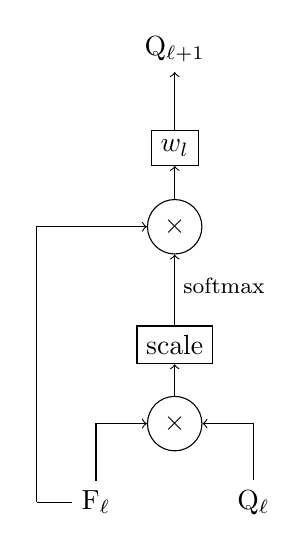
\begin{tikzpicture}
        \node (Q) at (4.5, -0.5) {Q$_\ell$};
        % \node (dimq) at (5, 0) {\scriptsize${1\times d_\ell}$};
        \node (F) at (2.5, -0.5) {F$_{\ell}$};
        % \node (dimft) at (3.0, -0) {\scriptsize${d_{\ell}\times p}$};
        \node (empt1) at (1.75, -0.5) {};
        \node[shape=circle,draw=black] (mm1) at (3.5, 0.5) {$\times$};
        % \node (dimraw) at (4,1) {\scriptsize$1\times p$};
        \node[shape=rectangle,draw=black](scale) at (3.5, 1.5) {scale};
        % \node (dimf) at (2.5, 3.175) {\scriptsize${p\times d_{\ell}}$};
        \node (soft) at (4.125, 2.25) {\footnotesize softmax};
        \node[shape=circle,draw=black] (mm2) at (3.5, 3) {$\times$};
        % \node[shape=rectangle,draw=black](project) at (3.5, 4) {$w_l: d_\ell\times d_{\ell+1}$ };
        \node[shape=rectangle,draw=black](project) at (3.5, 4) {$w_l$};
        % \node (dimscaled) [] at (4.25, 3.5) {\scriptsize $1\times d_\ell$};
        % \node [shape=circle,draw=black](sum1) at (3.5, 4) {+};
        % \node [shape=rectangle,draw=black](norm) at (3.5, 5.75) {LayerNorm};
        \node (Qplus1) at (3.5, 5.25) {Q$_{\ell+1}$};
        % \node (dimql) [align=left] at (4.25, 4.75) {\scriptsize$1\times d_{\ell+1}$};
        % \node (empt2) at (5.75, -0.5) {};

        \draw[->] (Q) |- node {} (mm1);
        \draw[->] (F) |- node {} (mm1);
        % \draw[-] (Q) -| node {} (empt2);
        % \draw[->] (empt2.center) |- node {} (sum1);
        \draw[->] (mm1) -- node {} (scale);
        \draw[->] (scale) -- node {} (mm2);
        \draw[-] (F) -| node {} (empt1.center);
        \draw[->] (empt1.center) |- node {} (mm2);
        \draw[->] (mm2) -- node {} (project);
        % \draw[->] (sum1) -- node {} (project);
        \draw[->] (project) -- node {} (Qplus1);
        % \draw[->] (norm) -- node {} (Qplus1);
    \end{tikzpicture}
    \caption{\textbf{Cross Attention Block}. We denote matrix multiplication as "$\otimes$". The softmax operation is performed on each row). For a given layer $\ell$ we update our [CLS] token $Q_\ell$; by computing its scaled cross attention with the feature maps $F_\ell$, that are then projected to the channel dimension in the following stage, using a dense layer parametrized by $w_\ell$.}
    \label{fig:fig_crossatt}
\end{figure}
